\chapter{Unsupervised Clustering Matching Using Nonlinear Feature Mapping}

\section{The model}

Based on the Iwatta's paper (see \cite{Iwata13,Iwata16}), we develop a non linear model for shape correspondence analysis using probabilistic latent variable models.

Suppose that we are given objects in $D$ domains $\mathcal{X}=\left\{\setObj\right\}_{d=1}^D$ mapped to a Hilbert space $\mathcal{H}_d$, where $\setObj = \left\{\phixnd\right\}_{n=1}^{N_d}$ is a set of objects in the $d$th domain, and $\phixnd \in \mathbb{R}^{M_d}$ is  the feature vector of the $n$th object in the $d$th domain. By introducing a basis function $\phi:x \mapsto \mathbb{R}$, that performs a given feature mapping over the objects, $\phi : \mathbf{X}_d\to\mathcal{H}_d$ such that $\forall x,x' \in \mathcal{X}$,\\

we can cluster groups of correspondences by using a basis function that represents the shape descriptors in the Hilbert space.

Our notation is summarized in Table \ref{tab:notf}. Note that we are unaware of any correspondence between objects in different domains. The number of objects $N_d$ and the dimensionality $L_d$ for each domain in $\mathcal{H}$ can be different from those of other domains.  Therefore, our task is to match clusters of descriptors (groupwise correspondences) across multiple brain structures in an
unsupervised manner \cite{Iwata16}.

\begin{table}
	\centering
	\caption{Notation.}
	\label{tab:notf}
	\resizebox{\textwidth}{!}{
		\begin{tabular}{l l l}
			\hline
			Symbol in $\mathcal{I}$& Symbol in $\mathcal{H}$  & Description \\
			\hline
			$D$ & &Number of shapes \\
			$N_d$ && Number of objects ($3D$-landmarks) in the $d$th shape\\
			$M_d$ &$L_d$& Dimensionality of the observed features in the $d$th shape\\
			 & $K$ & Dimensionality of a latent vector\\
			 & $J$ & Number of correspondences (latent vectors) to which objects are assigned\\
			$\phixnd$ & $\phixnd$ & Observation of the $n$th object in the $d$th shape, $\phixnd \in \mathbb{R}^{M_d}$\\
			  &$\mathbf{z}_j$& Latent vector for the $j$th correspondence, $\mathbf{z}_j \in \mathbb{R}^{K}$ \\
			 &$\mathbf{W}_d $& Projection matrix for the $d$th domain, $\mathbf{W}_d \in \mathbb{R}^{M_d \times K}$ \\
			$\mixwe$ && Mixture weight for the  $j$th cluster, $\mixwe \ge 0$, $\sum_{j=1}^{\infty}{\mixwe} = 1$\\
			\hline
			\hline 
		\end{tabular}}
	\end{table}
	
	
	As in infinite Gaussian mixture models, our approach assumes that there are an infinite number of clusters related to each
	correspondence, and each cluster $j$ has a latent vector $\lvecI\in \mathbb{R}^K$ in a latent space of dimension $K$. Descriptors that have the same cluster assignments $s_{dn}$ are related by the same latent vector and considered to match (establish a groupwise correspondence).
	
	Each object in $\phixnd \in \mathcal{H}_d$ in the $d$th domain is generated depending on the domain-specific projection matrix $\projMatI \in \mathbb{R}^{L_d \times K}$ and latent vector $\lvecsI$ that is selected from a set of latent vectors $\Z = \left\{\lvecI\right\}_{j=1}^\infty$. Here, $s_{dn}=\left\{1,\dots,\infty\right\}$ is the latent cluster assignment of object $\phixnd$.
	
	
	The proposed model is based on an infinite mixture model, where the
	probability of descriptor mapped in a Hilbert space $\phixnd$ is given by
	
	\begin{equation}
	p\left( {{\phixnd}|{\Z},{\boldsymbol{{W}}},{\boldsymbol{\theta }}} \right) = \sum\limits_{j = 1}^\infty  {{\theta _j}\mathcal{N}\left(\phixnd|\projMatI\lvecI,\alpha^{-1}\mathbf{I}\right)}, 
	\label{eq:llNLmodelf}
	\end{equation}
	
	where $\boldsymbol{{W}} = \left\{\projMatI\right\}_{d=1}^{D}$ is a set of projections
	matrices, $\boldsymbol{\theta}=\left(\theta_j\right)_{j=1}^{\infty}$
	are the mixture weights, $\theta_j$ represents the probability that
	the $j$th cluster is chosen, and
	$\mathcal{N}\left(\boldsymbol{\mu},\boldsymbol{\Sigma}\right)$ denotes
	a normal distribution with mean $\boldsymbol{\mu}$ and covariance
	matrix $\boldsymbol{\Sigma}$. One important contribution derived in \cite{Iwata13}, is that we can analyze multiples structures with different properties and dimensionalities, by employing projection matrices for each brain structure (domain-specific). Figure
	\ref{fig:pipelinef} shows the scheme of the proposed model, in which
	the relationship between shape descriptors, and
	latent vectors is described.
	
	\begin{figure}[h!]
		\centering
		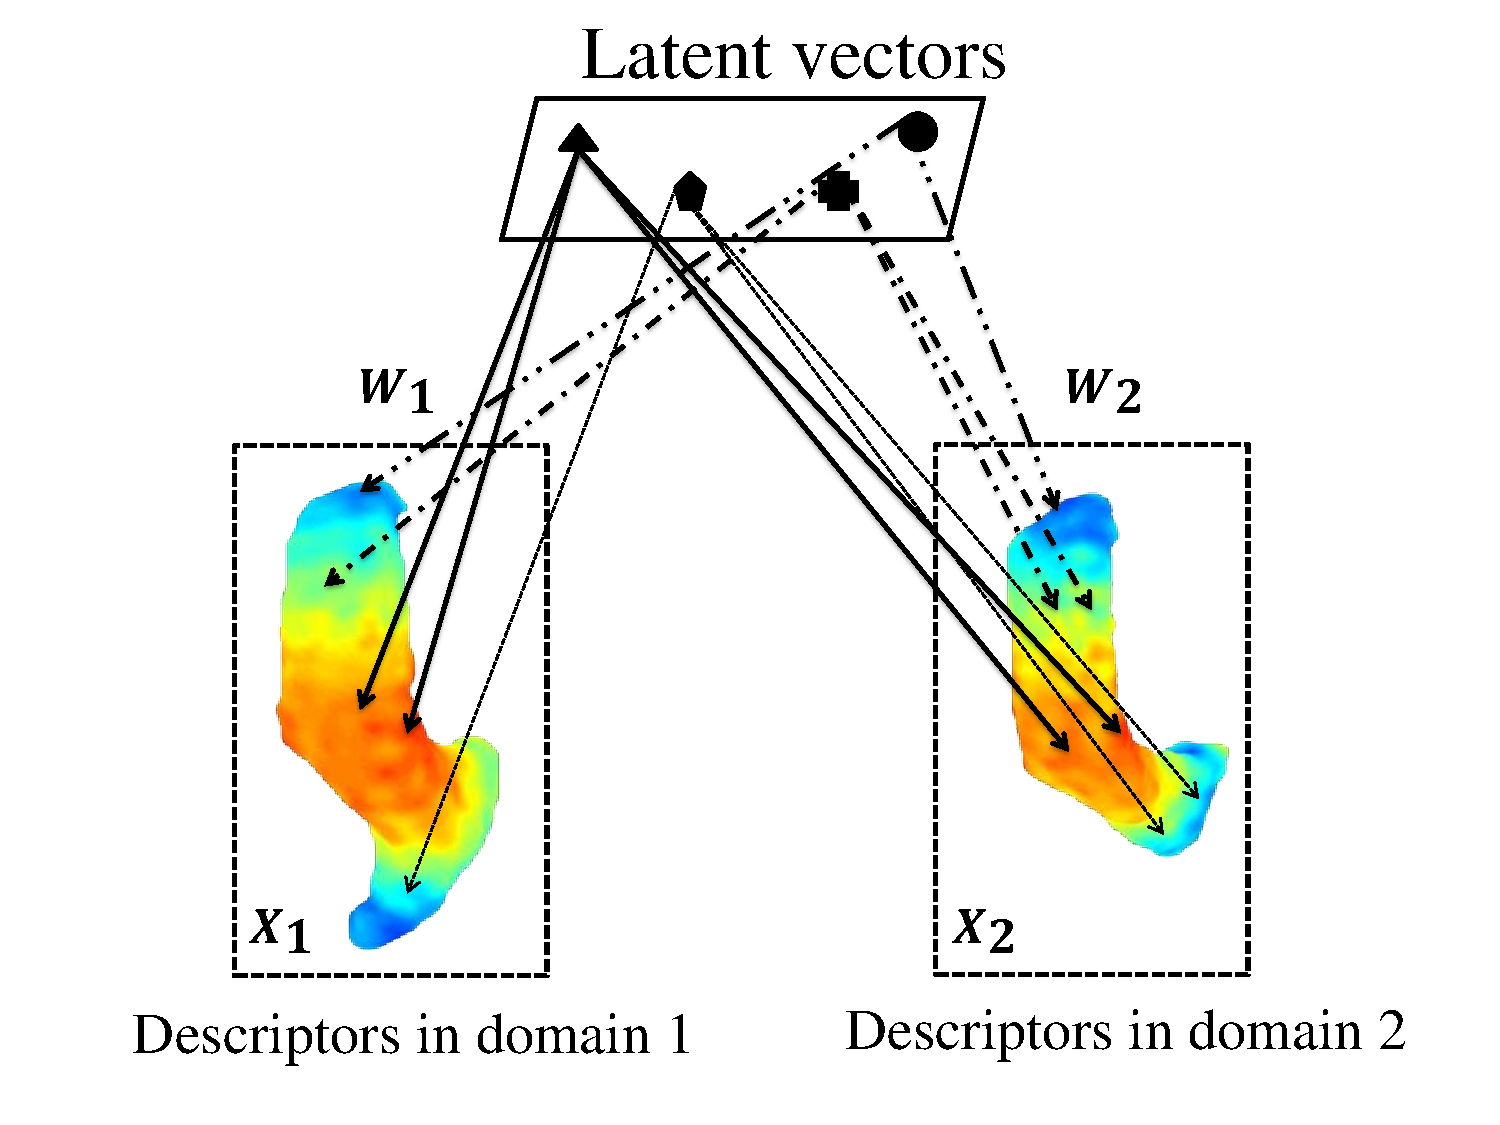
\includegraphics[width=0.6\textwidth]{img/pipelineGroupCorr}
		\caption{Scheme for the groupwise correspondence method. The
			figure shows an example of establishing clusters of correspondences
			in two domains (left ventrals).}
		\label{fig:pipelinef}
	\end{figure} 
	
	In order to draw the cluster proportions, we use a stick-breaking process to generate mixture weights for a Dirichlet process with
	concentration parameter $\gamma$ \cite{Iwata13} ($a$,$b$ and $r$ are the hyperparameters). The joint probability
	of the data $\boldsymbol{\Phi}$, and the cluster assignments
	$\mathbf{S}=\left\{\left\{s_{dn}\right\}_{n=1}^{N_{d}}\right\}_{d=1}^{D}$
	are given by
	\begin{equation}
	p\left(\boldsymbol{\Phi},\mathbf{S}|\boldsymbol{{W}},a,b,r,\gamma\right)=
	p\left(\mathbf{S}|\gamma\right)p\left(\boldsymbol{\Phi}|\mathbf{S},\boldsymbol{{W}},a,b,r\right).
	\label{eq:jointPf}
	\end{equation}
	
	
	By marginalizing out the mixture weights $\boldsymbol{\theta}$, $p\left(\mathbf{S}|\gamma\right)$ becomes in
	\begin{equation}
	p\left(\mathbf{S}|\gamma\right) =\frac{\gamma^{J}\prod\limits_{j=1}^{J}{\left(N_{.j}-1\right)!}}{\gamma\left(\gamma+1\right)\dots\left(\gamma+N-1\right)},
	\end{equation}
	where $N=\sum\limits_{d=1}^{D}N_d$ is the total number of shape
	descriptors, $N_{.j}$ represents the number of descriptors assigned to
	the cluster $j$, and $J$ is the number of clusters that satisfies
	$N_{.j}>0$. 
	
	\subsection{Likelihood for the proposed model}
	By marginalizing out latent vectors $\mathbf{Z}$ and the
	precision parameter $\alpha$, the second factor of \eqref{eq:jointPf} is
	computed by
	
	\begin{align}
	p\left(\setXphi|\Scluster,\WIn,a,b,r\right) &=  \int \int \prod_{d=1}^{D}\prod_{n=1}^{N_d}{\gD{\phixnd|\projMatI \lvecsI}{\alpha^{-1}\eye}\catD{\alpha|a}{b}} \times \prod_{j=1}^{J}\gD{\lvecI|\mathbf{0}}{\left(\alpha r\right)^{-1}\eye}d\Z d\alpha  \notag \\
	&=\int \int \prod_{d=1}^{D}\prod_{n=1}^{N_d}\left(\frac{\alpha}{2\pi}\right)^{M_d /2}\exp\left(-\frac{\alpha}{2}||\phixnd-\projMatI\lvecsI||^2\right) \prod_{j=1}^{J}\left(\frac{\alpha r}{2\pi}\right)^{K/2} \notag \\
	&\times \exp\left(-\frac{\alpha r}{2}||\lvecI||^2\right)\frac{b^a \alpha^{a-1}}{\gammaA}\exp\left(-b\alpha\right)d\Z d\alpha \notag\\
	&=\frac{b^a}{\gammaA}\int \int \left(\frac{\alpha}{2\pi}\right)^{\sum_d M_d N_d /2}\exp\left(-\frac{\alpha}{2} \sum_{d=1}^{D}\sum_{n=1}^{N_d}||\phixnd-\projMatI\lvecsI||^2\right)\left(\frac{\alpha r}{2\pi}\right)^{KJ/2} \notag \\
	&\times \exp\left(-\frac{\alpha r}{2} \sum_{j=1}^{J}||\lvecI||^2\right)\exp\left(-b\alpha\right)\alpha^{a-1}d\Z d\alpha 
	\label{eq:llnmlinf}
	\end{align}
	
	
	Solving for the first exponential term
	
	\begin{align}
	\exp\left(-\frac{\alpha}{2} \sum_{d=1}^{D}\sum_{n=1}^{N_d}||\phixnd-\projMatI\lvecsI||^2\right) &= \exp\Big(-\frac{\alpha}{2} \sum_{d=1}^{D}\sum_{n=1}^{N_d}\big[ \phixnd^\top \phixnd  \notag\\
	&  - 2 \lvecsI ^\top \projMatI^\top \phixnd + \lvecsI^\top \projMatI^\top \projMatI \lvecsI \big]\Big) \notag\\
	%&=  \exp\Big(-\frac{\alpha}{2} \sum_{d=1}^{D}\sum_{n=1}^{N_d}\big[ \kernel{\phixnd}{\phixnd}  \notag\\
	%&  - 2 \lvecs ^\top\underbrace{ \projMat^\top \phixnd }_{A}+ \lvecs^\top \underbrace{\projMat^T \projMat}_{B} \lvecs \big]\Big)
	\label{eq:exp_XWzlinf}
	\end{align}
	
	The equation in \eqref{eq:llnmlinf} becomes
	
	\begin{align}
	p\left(\setXphi|\Scluster,\WIn,a,b,r\right) &= \frac{b^a}{\gammaA}\int \int \left(\frac{\alpha}{2\pi}\right)^{\sum_d M_d N_d /2}\exp\Big(-\frac{\alpha}{2} \sum_{d=1}^{D}\sum_{n=1}^{N_d}\big[ \phixnd^\top \phixnd  \notag\\
	&  - 2 \lvecsI ^\top \projMatI^\top \phixnd + \lvecsI^\top \projMatI^\top \projMatI \lvecsI \big]\Big)\left(\frac{\alpha r}{2\pi}\right)^{KJ/2} \notag \\
	&\times \exp\left(-\frac{\alpha r}{2} \sum_{j=1}^{J}\lvecI^\top\lvecI\right)\exp\left(-b\alpha\right)\alpha^{a-1}d\Z d\alpha.
	\label{eq:llnmlin2f}
	\end{align}
	
	The exponential terms in \eqref{eq:llnmlin2f} becomes
	
	\begin{align}
	&\exp\Bigg(-\frac{\alpha}{2} \sum_{d=1}^{D}\sum_{n=1}^{N_d}\big[ \phixnd^\top \phixnd-2 \lvecsI ^\top \projMatI^\top \phixnd + \lvecsI^\top \projMatI^\top \projMatI \lvecsI\big]-\frac{\alpha r}{2} \sum_{j=1}^{J}\lvecI^\top\lvecI -b\alpha\Bigg) = \notag\\
	& \exp\Bigg(-\frac{\alpha}{2} \sum_{d=1}^{D}\sum_{n=1}^{N_d}\big[ \phixnd^\top \phixnd-b\alpha\Bigg)\exp\Bigg(-\frac{\alpha}{2} \sum_{d=1}^{D}\sum_{n=1}^{N_d}\big[ -2 \lvecsI ^\top \projMatI^\top \phixnd+\lvecsI^\top \projMatI^\top \projMatI \lvecsI\big] \notag\\
	&-\frac{\alpha r}{2} \sum_{j=1}^{J}\lvecI^\top\lvecI\Bigg) \label{eq:llKernelExp1linf}
	\end{align}
	
	By analyzing the $n$th objects that has the cluster assignment $j$ ($n:s_{dn}=j$), the second factor in \eqref{eq:llKernelExp1linf} becomes
	
	\begin{align}
	&\exp\Bigg(-\frac{\alpha}{2} \sum_{d=1}^{D}\sum_{n=1}^{N_d}\big[ -2 \lvecsI ^\top \projMatI^\top \phixnd+\lvecsI^\top \projMatI^\top \projMatI \lvecsI \big] -\frac{\alpha r}{2} \sum_{j=1}^{J}\lvecI^\top\lvecI \Bigg) = \exp\Bigg(-\frac{\alpha}{2} \sum_{d=1}^{D}\sum_{n:s_{dn}\ne j}\big[  -2 \lvecsI ^\top \projMatI^\top \phixnd\notag\\
	&+ \lvecsI^\top \projMatI^\top \projMatI \lvecsI \big] \Bigg)\times \underbrace{\exp\Bigg(-\frac{\alpha}{2} \sum_{d=1}^{D}\sum_{n:s_{dn}=j}\big[ -2 \lvecsI ^\top \projMatI^\top \phixnd+\lvecsI^\top \projMatI^\top \projMatI \lvecsI \big]-\frac{\alpha r}{2} \sum_{j=1}^{J}\lvecI^\top\lvecI\Bigg)}_{C} \notag\\
	&=\exp\Bigg(-\frac{\alpha}{2} \sum_{d=1}^{D}\sum_{j=1}^J N_{dj}\big[ -2 \lvecI ^\top \projMatI^\top \phixnd+\lvecI^\top \projMatI^\top \projMatI \lvecI \big]-\frac{\alpha r}{2} \sum_{j=1}^{J}\lvecI^\top\lvecI\Bigg) \notag\\
	&=\exp\Bigg(-\frac{\alpha}{2} \sum_{d=1}^{D}\sum_{j=1}^J \big[ -2 \lvecI ^\top \projMatI^\top \sum_{n:s_{dn}=j}\phixnd+\lvecI^\top N_{dj}\projMatI^\top \projMatI \lvecI \big]-\frac{\alpha r}{2} \sum_{j=1}^{J}\lvecI^\top\lvecI\Bigg) \notag \\
	&=\exp\Bigg(-\frac{\alpha}{2}\sum_{j=1}^J \big[ -2 \lvecI ^\top  \sum_{d=1}^{D}\projMatI^\top \sum_{n:s_{dn}=j}\phixnd+\lvecI^\top  \sum_{d=1}^{D} N_{dj}\projMatI^\top \projMatI \lvecI \big]-\frac{\alpha r}{2} \sum_{j=1}^{J}\lvecI^\top\lvecI\Bigg) \notag \\
	&= \exp\Bigg(-\frac{\alpha}{2}\sum_{j=1}^J \big[ -2 \lvecI ^\top  \sum_{d=1}^{D}\projMatI^\top \sum_{n:s_{dn}=j}\phixnd+\lvecI^\top  \sum_{d=1}^{D} N_{dj}\projMatI^\top \projMatI \lvecI + r\lvecI^\top\lvecI\big]\Bigg) \notag \\
	&= \exp\Bigg(-\frac{\alpha}{2}\sum_{j=1}^J \big[ -2 \lvecI ^\top  \sum_{d=1}^{D}\projMatI^\top \sum_{n:s_{dn}=j}\phixnd+\lvecI^\top  \left(\sum_{d=1}^{D} N_{dj}\projMatI^\top \projMatI + r\eye\right) \lvecI \big]\Bigg).
	\label{eq:llExp1linf}
	\end{align}
	
	By using the quadratic property
	
	\begin{align}
	-\frac{1}{2}\left(\mathbf{z}-\boldsymbol{\mu}\right)^\top \boldsymbol{C}^{-1} \left(\mathbf{z}-\boldsymbol{\mu}\right) = -\frac{1}{2}\left[\mathbf{z}^\top \boldsymbol{C}^{-1}\mathbf{z} -2\mathbf{z}^\top \boldsymbol{C}^{-1}\boldsymbol{\mu} + \boldsymbol{\mu}^\top\boldsymbol{C}^{-1}\boldsymbol{\mu}\right] \label{eq:quadlinf},
	\end{align}
	
	where 
	
	\begin{align}
	\Cin^{-1} = \sum_{d=1}^{D} N_{dj}\projMatI^\top \projMatI + r\eye,
	\end{align}
	
	and
	
	\begin{align}
	-2\mathbf{z}^\top \boldsymbol{C}^{-1}\boldsymbol{\mu} &=  -2 \lvecI ^\top  \sum_{d=1}^{D}\projMatI^\top \sum_{n:s_{dn}=j}\phixnd \notag \\
	\muJ &= \Cin  \sum_{d=1}^{D}\projMatI^\top \sum_{n:s_{dn}=j}\phixnd .
	\end{align}
	
	By completing the square as: $\textrm{arg} = \textrm{arg} + \frac{1}{2}\boldsymbol{\mu}^\top\boldsymbol{C^{-1}}\boldsymbol{\mu} -\frac{1}{2}\boldsymbol{\mu}^\top\boldsymbol{C^{-1}}\boldsymbol{\mu}$, the argument in \eqref{eq:llExp1lin} becomes
	
	\begin{align}
	&\exp\Bigg(-\frac{\alpha}{2}\sum_{j=1}^J \big[ -2 \lvecI ^\top  \sum_{d=1}^{D}\projMatI^\top \sum_{n:s_{dn}=j}\phixnd+\lvecI^\top  \left(\sum_{d=1}^{D} N_{dj}\projMatI^\top \projMatI + r\eye\right) \lvecI \big]\Bigg) \notag\\ &= \exp\Bigg(-\frac{\alpha}{2}\Big[\sum_{j=1}^{J} \left(\lvecI-\muJ\right)^\top\Cin^{-1}\left(\lvecI-\muJ\right)\Big]\Bigg)
	\exp\Bigg(-\frac{\alpha}{2}\sum_{j=1}^{J}\muJ^\top\Cin^{-1}\muJ\Bigg) \label{eq:expFinalKernlinf}
	\end{align}
	
	
	Substituting \eqref{eq:expFinalKernlinf} in \eqref{eq:llnmlin2} give us
	
	\begin{align}
	p\left(\mathbf{X}|\Scluster,\WIn,a,b,r\right)&=\frac{b^a}{\gammaA}\iint \left(\frac{\alpha}{2\pi}\right)^{\sum_d M_d N_d /2}\left(\frac{\alpha r}{2\pi}\right)^{KJ/2}\exp\Bigg(-\frac{\alpha}{2}\Big[\sum_{j=1}^{J} \left(\lvecI-\muJ\right)^\top\Cin^{-1}\left(\lvecI-\muJ\right)\Big]\Bigg)d\Z \notag\\
	&\exp\Bigg(-\alpha\Bigg[\frac{1}{2} \sum_{d=1}^{D}\sum_{n=1}^{N_d}\phixnd^\top \phixnd  -\frac{1}{2}\sum_{j=1}^{J}\muJ^\top\Cin^{-1}\muJ +b \Bigg]\Bigg)\alpha^{a-1}d\alpha \label{eq:llFinalIntegralslinf}
	\end{align}
	
	In equation \eqref{eq:llFinalIntegralslinf}, factors related to $\Z$ are grouped together. We integrated out $\Z$ using
	
	\begin{align}
	\int \exp\left(-\frac{1}{2}\left(\lvecI-\muJ\right)^\top\left[\alpha^{-1}\Cin\right]^{-1}\left(\lvecI-\muJ\right)\right)d\lvecI = \left(2\pi\right)^{K/2}|\alpha^{-1}\Cin|^{1/2} = \left(2\pi\right)^{K/2}\alpha^{-K/2}|\Cin|^{1/2},
	\end{align}
	
	which is the normalization constant of $P$-dimensional Gaussian distribution. Since we have the sum over the number of correspondences (latent vectors), $K$, the above equation ranges for all of these clusters. The equation \eqref{eq:llFinalIntegralslin}, becomes
	
	\begin{align}
	p\left(\setXphi|\Scluster,\WIn,a,b,r\right) &=\frac{b^a}{\gammaA}\int \left(\frac{\alpha}{2\pi}\right)^{\sum_d M_d N_d /2}\left(\frac{\alpha r}{2\pi}\right)^{KJ/2} \prod_{j=1}^{J}\Big[\left(2\pi\right)^{K/2}\alpha^{-K/2}|\Cin|^{1/2}\Big]
	\notag\\
	&\exp\Bigg(-\alpha\Bigg[\frac{1}{2} \sum_{d=1}^{D}\sum_{n=1}^{N_d}\phixnd^\top \phixnd -\frac{1}{2}\sum_{j=1}^{J}\muJ^\top\Cin^{-1}\muJ +b \Bigg]\Bigg)\alpha^{a-1}d\alpha \\
	&=\frac{b^a}{\gammaA}\int \left(\frac{\alpha}{2\pi}\right)^{\sum_d M_d N_d /2}\left(\frac{\alpha r}{2\pi}\right)^{KJ/2} \left(2\pi\right)^{KJ/2}\alpha^{-KJ/2}\prod_{j=1}^{J}|\Cin|^{1/2} \notag\\
	&\exp\Bigg(-\alpha\Bigg[\frac{1}{2} \sum_{d=1}^{D}\sum_{n=1}^{N_d}\phixnd^\top\phixnd -\frac{1}{2}\sum_{j=1}^{J}\muJ^\top\Cin^{-1}\muJ +b \Bigg]\Bigg)\alpha^{a-1}d\alpha\label{eq:llFinalIntegralZlinf}
	\end{align}
	
	The $\alpha$ parameter is integrated out by using the following normalization constant of a Gamma distribution 
	\begin{align}
	\int \alpha^{a'-1}\exp\left(-b\alpha\right)d\alpha = \frac{\Gamma\left(a'\right)}{b'^{a'}}.
	\end{align}
	
	Finally the likelihood is given by
	
	\begin{align}
	p\left(\setXphi|\Scluster,\WIn,a,b,r\right) &=\left(2\pi\right)^{-\frac{\sum_d M_d N_d}{2}}r^{\frac{KJ}{2}}\frac{b^{a}}{b'^{a'}}\frac{\Gamma\left(a'\right)}{\Gamma\left(a\right)}\prod_{j=1}^{J}|\Cin|^{1/2},
	\label{eq:llFinalIntegrallastlinf}
	\end{align}
	
	Here,
	
	\begin{align}
	a'=a+{\frac{\Sigma_d M_d N_d}{2}}, \quad \quad b'=b+{\frac{1}{2}}\sum\limits_{d=1}^{D}\sum\limits_{n=1}^{N_d}{\phixnd^{\top}\phixnd}-{\frac{1}{2}}\sum\limits_{j=1}^{J}\boldsymbol{\mu}_j^\top \mathbf{C}_j^{-1}\boldsymbol{\mu}_j,
	\end{align}
	\begin{align}
	\boldsymbol{\mu}_j =\mathbf{C}_j\sum\limits_{d=1}^{D}{\mathbf{W}_d^\top\sum\limits_{n:s_{dn}=j}{\phixnd}}, \quad \quad \mathbf{C}_{j}^{-1} =\sum\limits_{d=1}^{D}{N_{dj}\mathbf{W}_d^\top\mathbf{W}_d+r\mathbf{I}},
	\end{align}
	
	where $N_{dj}$ is the number of descriptors assigned to cluster $j$ in the shape $d$ (domain). 
	
	\subsection{Inference for the Linear Model}
	
	\subsubsection{M-Step Linear}
	
	In the M-step, the projection matrices $\WIn$ are estimated by maximizing the logarithm of the joint likelihood \eqref{eq:jointP}. The gradient of the joint likelihood is computed by
	
	\begin{align}
	\frac{\partial \log p\left(\boldsymbol{\Phi},\mathbf{S}|\WIn,a,b,r,\gamma\right)}{\partial\projMatI} =
	\frac{\partial \log p\left(\mathbf{S}|\gamma\right)}{\partial\projMatI} + \frac{\partial \log p\left(\boldsymbol{\Phi}|\mathbf{S},\boldsymbol{\mathbf{W}},a,b,r\right)}{\partial\projMatI},
	\end{align}
	
	Since the derivative of the first term in the above expression is zero, the expression becomes
	
	\begin{align}
	\frac{\partial \log p\left(\setXphi,\mathbf{S}|\WIn,a,b,r,\gamma\right)}{\partial\projMatI} &=
	\frac{\partial \log p\left(\setXphi|\mathbf{S},\WIn,a,b,r\right)}{\partial\projMatI} = \frac{\partial \log \Big[\left(2\pi\right)^{-\frac{\sum_d M_d N_d}{2}}r^{\frac{JK}{2}}\frac{b^{a}}{b'^{a'}}\frac{\Gamma\left(a'\right)}{\Gamma\left(a\right)}\prod_{j=1}^{J}|\Cin|^{1/2}\Big]}{\partial\projMat},\notag\\
	&= \frac{\partial \log \Big[\frac{cte}{b'^{a'}} \prod_{j=1}^{J}|\Cin|^{1/2}\Big]}{\partial\projMatI}\notag,\\
	& = -\frac{a'}{b'}\frac{\partial b'}{\dWjIn}+\frac{1}{2}\sum_{j=1}^{J}\frac{\partial \log |\Cin|}{\dWjIn}+0 , \notag \\
	& =  -\frac{a'}{b'}\frac{\partial b'}{\dWjIn}+\frac{1}{2}\sum_{j=1}^{J} \operatorname{tr}\left(\Cin^{-1}\frac{\partial \Cin}{\dWjIn}\right)
	%\label{eq:derivativeW1}
	\end{align}
	
	where
	
	\begin{align}
	\frac{\partial b'}{\dWjIn} = \frac{\partial}{\dWjIn}\Big[ \frac{1}{2} \sum_{d=1}^{D}\sum_{n=1}^{N_d}\phixnd^\top\phixnd -\frac{1}{2}\sum_{j=1}^{J}\muJ^\top\Cin^{-1}\muJ +b \Big],
	\end{align}
	
	Here the second factor of the argument is the only which depends on $\projMat$.
	%\C\sum\limits_{d=1}^{D}{\sum\limits_{n:s_{dn}=j}\kawx}
	\begin{align}
	\frac{\partial b'}{\dWjIn} &= \frac{\partial}{\dWjIn}\Big[-\frac{1}{2}\sum_{j=1}^{J}\muJ^\top\Cin^{-1}\muJ \Big] \notag \\
	&=-\frac{1}{2}\sum_{j=1}^{J}\frac{\partial}{\dWjIn}\Big[\muJ^\top\Cin^{-1}\muJ \Big] =-\frac{1}{2}\sum_{j=1}^{J}\tr\left(\frac{\partial}{\dWjIn}\Big[\muJ^\top\Cin^{-1}\muJ \Big]\right) \notag \\
	&=-\frac{1}{2}\sum_{j=1}^{J}\tr\left(\frac{\partial \muJ^\top}{\dWjIn}\Cin^{-1}\muJ + \muJ^\top\left(\frac{\partial \Cin^{-1}}{\dWjIn}\muJ+\Cin^{-1}\frac{\partial \muJ}{\dWjIn}\right)\right) \notag \\
	& = -\frac{1}{2}\sum_{j=1}^{J} \tr\left(\partial \muJ^\top\Cin^{-1}\muJ\right) + \tr\left( \muJ^\top\partial\Cin^{-1}\muJ\right) + \tr\left( \muJ^\top\Cin^{-1}\partial\muJ\right),
	\end{align}
	
	by applying trace properties (transpose elements)
	
	\begin{align}
	\frac{\partial b'}{\dWjIn} &= -\frac{1}{2}\sum_{j=1}^{J} \tr\left(\partial \muJ^\top\Cin^{-1}\muJ\right) + \tr\left( \muJ^\top\partial\Cin^{-1}\muJ\right) + \tr\left( \muJ^\top\Cin^{-1}\partial\muJ\right) \notag \\
	&=  -\frac{1}{2}\sum_{j=1}^{J} \tr\left( \muJ^\top\Cin^{-1}\partial\muJ\right) + \tr\left( \muJ^\top\partial\Cin^{-1}\muJ\right) + \tr\left( \muJ^\top\Cin^{-1}\partial\muJ\right) \notag \\
	&= -\frac{1}{2}\sum_{j=1}^{J} \tr\left( \muJ^\top\partial\Cin^{-1}\muJ\right) + 2\tr\left( \muJ^\top\Cin^{-1}\partial\muJ\right) \notag\\
	&=  \underbrace{-\sum_{j=1}^{J}\tr\left( \muJ^\top\Cin^{-1}\partial\muJ\right)}_{A} \underbrace{-\frac{1}{2}\sum_{j=1}^{J} \tr\left( \muJ^\top\partial\Cin^{-1}\muJ\right)}_{B} 
	\end{align}
	
	First, for the B part we have:
	
	% % % % % % % % % % % % % % % % % % % % % % % % % % %
	
	
	\begin{align}
	-\frac{1}{2}\sum_{j=1}^{J} \tr\left( \muJ^\top\partial\Cin^{-1}\muJ\right) &= -\frac{1}{2}\sum_{j=1}^{J} \tr\left( \muJ^\top\partial\left[\sum_{d=1}^{D}N_{dj}\projMatI^\top\projMatI+r\mathbf{I}\right]\muJ\right) \notag \\
	&=  -\frac{1}{2}\sum_{j=1}^{J} \tr\left( \muJ^\top\left[N_{dj}\left(\partial\projMatI^\top\projMatI+\projMatI^\top\partial\projMatI\right)\right]\muJ\right) \notag \\
	&=  -\frac{1}{2}\sum_{j=1}^{J} \left[N_{dj}\tr\left( \muJ^\top\partial\projMatI^\top\projMatI\muJ\right)+N_{dj}\tr\left(\muJ^\top\projMatI^\top\partial\projMatI\muJ\right)\right] \notag \\
	&=  -\frac{1}{2}\sum_{j=1}^{J} \left[N_{dj}\tr\left( \left(\muJ^\top\partial\projMatI^\top\projMatI\muJ\right)^\top\right)+N_{dj}\tr\left(\muJ\muJ^\top\projMatI^\top\partial\projMatI\right)\right] \notag\\
	&=  -\frac{1}{2}\sum_{j=1}^{J} \left[N_{dj}\tr\left( \muJ\muJ^\top\projMatI^\top\partial\projMatI\muJ\right)+N_{dj}\tr\left(\muJ\muJ^\top\projMatI^\top\partial\projMatI\right)\right] \notag\\
	&=  -\sum_{j=1}^{J} N_{dj}\tr\left( \muJ\muJ^\top\projMatI^\top\partial\projMatI\right).
	\label{eq:partBLinearMstepf}
	\end{align}
	
	
	By using derivatives properties for trace forms as 
	\begin{align}
	\frac{\partial \tr\left[F\left(\boldsymbol{\Phi}\right)\right]}{\partial \boldsymbol{\Phi}} = f\left(\boldsymbol{\Phi}\right)^\top,
	\end{align}
	
	where $f\left(\cdot\right)$ is the scalar derivative of $F\left(\cdot\right)$, the equation \eqref{eq:partBLinearMstep} becomes
	
	\begin{align}
	-\frac{1}{2}\sum_{j=1}^{J} \tr\left( \muJ^\top\partial\Cin^{-1}\muJ\right) &= -\sum_{j=1}^{J} N_{dj}\left( \muJ\muJ^\top\projMatI^\top\right)^\top =  -\sum_{j=1}^{J} N_{dj} \projMatI \muJ\muJ^\top.
	\end{align}
	
	Besides, for the A part we have:
	
	\begin{align}
	-\sum_{j=1}^{J}\tr\left( \muJ^\top\Cin^{-1}\partial\muJ\right) \rightarrow \frac{\partial \muJ}{\partial \projMatI} = \frac{\partial}{\partial \projMatI}\left[\Cin\sum_{d=1}^{D}\projMatI^\top\sum_{n:s_{dn}=j}\phixnd\right].
	\end{align}
	
	The derivative for $\muJ$ is given by
	
	\begin{align}
	\frac{\partial \muJ}{\partial \projMatI} &= \underbrace{\partial\Cin\left(\sum_{d=1}^{D}\projMatI^\top\sum_{n:s_{dn}=j}\phixnd\right)}_{C} + \underbrace{\Cin\partial\left(\sum_{d=1}^{D}\projMatI^\top\sum_{n:s_{dn}=j}\phixnd\right)}_{D} 
	\end{align}
	
	For the $C$ part, we have
	
	\begin{align}
	\partial\Cin\left(\sum_{d=1}^{D}\projMatI^\top\sum_{n:s_{dn}=j}\phixnd\right) &= \frac{\partial}{\partial \projMatI}\left[\left(\sum_{d=1}^{D}N_{dj}\projMatI^\top\projMatI+r\mathbf{I}\right)^{-1}\right]\left(\sum_{d=1}^{D}\projMatI^\top\sum_{n:s_{dn}=j}\phixnd\right) \notag \\
	&= -\Cin \frac{\partial}{\partial \projMatI}\left[\sum_{d=1}^{D}N_{dj}\projMatI^\top\projMatI+r\mathbf{I}\right]\Cin\sum_{d=1}^{D}\projMatI^\top\sum_{n:s_{dn}=j}\phixnd \notag\\
	&=-\Cin\left(N_{dj}\left[\partial\projMatI^\top\projMatI+\projMatI^\top\partial\projMatI\right]\right)\muJ.
	\end{align}
	
	The $D$ part is computed as
	
	\begin{align}
	\Cin\partial\left(\sum_{d=1}^{D}\projMatI^\top\sum_{n:s_{dn}=j}\phixnd\right) = \Cin\partial\projMatI^\top\sum_{n:s_{dn}=j}\phixnd.
	\end{align}
	
	Then the $A$ part becomes,
	
	\begin{align}
	-\sum_{j=1}^{J}\tr\left( \muJ^\top\Cin^{-1}\partial\muJ\right) &=-\sum_{j=1}^{J}\tr\left( \muJ^\top\Cin^{-1}\left[-\Cin\left(N_{dj}\left[\partial\projMatI^\top\projMatI+\projMatI^\top\partial\projMatI\right]\right)\muJ+\Cin\partial\projMatI^\top\sum_{n:s_{dn}=j}\phixnd\right]\right) \notag \\
	&= \sum_{j=1}^{J}N_{dj}\tr\left(\muJ^\top\Cin^{-1}\Cin\left(\partial\projMatI^\top\projMatI\right)\muJ\right) +  \sum_{j=1}^{J}N_{dj}\tr\left(\muJ^\top\Cin^{-1}\Cin\left(\projMatI^\top\partial\projMatI\right)\muJ\right) \notag\\
	&-\sum_{j=1}^{J}\tr\left(\muJ^\top\Cin^{-1}\Cin\partial\projMatI^\top\sum_{n:s_{dn}=j}\phixnd\right) \notag \\
	&= \sum_{j=1}^{J}N_{dj}\tr\left(\muJ^\top\partial\projMatI^\top\projMatI\muJ\right) +  \sum_{j=1}^{J}N_{dj}\tr\left(\muJ^\top\projMatI^\top\partial\projMatI\muJ\right) \notag\\
	&-\sum_{j=1}^{J}\tr\left(\muJ^\top\partial\projMatI^\top\sum_{n:s_{dn}=j}\phixnd\right) \notag \\
	&= \sum_{j=1}^{J}N_{dj}\tr\left(\left(\muJ^\top\partial\projMatI^\top\projMatI\muJ\right)^\top\right) +  \sum_{j=1}^{J}N_{dj}\tr\left(\muJ\muJ^\top\projMatI^\top\partial\projMatI\right) \notag\\
	&-\sum_{j=1}^{J}\tr\left(\left(\muJ^\top\partial\projMatI^\top\sum_{n:s_{dn}=j}\phixnd\right)^\top\right) \notag \\
	&= \sum_{j=1}^{J}N_{dj}\tr\left(\muJ^\top\projMatI^\top\partial\projMatI\muJ\right) +  \sum_{j=1}^{J}N_{dj}\tr\left(\muJ\muJ^\top\projMatI^\top\partial\projMatI\right) \notag\\
	&-\sum_{j=1}^{J}\tr\left(\sum_{n:s_{dn}=j}\phixnd^\top\partial\projMatI\muJ\right) \notag \\
	&= \sum_{j=1}^{J}N_{dj}\tr\left(\muJ\muJ^\top\projMatI^\top\partial\projMatI\right) +  \sum_{j=1}^{J}N_{dj}\tr\left(\muJ\muJ^\top\projMatI^\top\partial\projMatI\right) \notag\\
	&-\sum_{j=1}^{J}\tr\left(\muJ\sum_{n:s_{dn}=j}\phixnd^\top\partial\projMatI\right) \notag \\
	&= 2\sum_{j=1}^{J}N_{dj}\tr\left(\muJ\muJ^\top\projMatI^\top\partial\projMatI\right)-\sum_{j=1}^{J}\tr\left(\muJ\sum_{n:s_{dn}=j}\phixnd^\top\partial\projMatI\right) .
	\end{align}
	
	
	By using the derivatives properties for trace forms described above, we have
	
	\begin{align}
	-\sum_{j=1}^{J}\tr\left( \muJ^\top\Cin^{-1}\partial\muJ\right) &= 2\sum_{j=1}^{J}N_{dj}\left(\muJ\muJ^\top\projMatI^\top\right)^\top-\sum_{j=1}^{J}\left(\muJ\sum_{n:s_{dn}=j}\phixnd^\top\right)^\top \notag \\
	&= 2\sum_{j=1}^{J}N_{dj}\projMatI\muJ\muJ^\top - \sum_{j=1}^{J}\sum_{n:s_{dn}=j}\phixnd \muJ^\top .
	\end{align}
	
	Finally 
	
	\begin{align}
	\frac{\partial b'}{\dWjIn} &= 2\sum_{j=1}^{J}N_{dj}\projMatI\muJ\muJ^\top - \sum_{j=1}^{J}\sum_{n:s_{dn}=j}\phixnd \muJ^\top -  -\sum_{j=1}^{J} N_{dj} \projMatI \muJ\muJ^\top \notag \\
	&= \sum_{j=1}^{J}N_{dj}\projMatI\muJ\muJ^\top - \sum_{j=1}^{J}\sum_{n:s_{dn}=j}\phixnd \muJ^\top \notag \\
	&= \sum_{j=1}^{J}\left\{N_{dj}\projMatI\muJ\muJ^\top - \sum_{n:s_{dn}=j}\phixnd \muJ^\top\right\}.
	\end{align}
	
	For the part $B$,
	
	\begin{align}
	\frac{1}{2}\sum_{j=1}^{J} \operatorname{Tr}\left(\Cin^{-1}\frac{\partial \Cin}{\dWjIn}\right) &= \frac{1}{2}\sum_{j=1}^{J} \operatorname{tr}\left(\Cin^{-1}\left(-\Cin\left(N_{dj}\left[\partial\projMatI^\top\projMatI+\projMatI^\top\partial\projMatI\right]\right)\Cin\right)\right) \notag \\
	&= -\frac{1}{2}\sum_{j=1}^{J}N_{dj}\operatorname{tr}\left(\Cin^{-1}\Cin\left[\partial\projMatI^\top\projMatI+\projMatI^\top\partial\projMatI\right]\Cin\right) \notag \\
	&= -\frac{1}{2}\sum_{j=1}^{J}N_{dj}\operatorname{tr}\left(\Cin^{-1}\Cin\left[\partial\projMatI^\top\projMatI+\projMatI^\top\partial\projMatI\right]\Cin\right) \notag \\
	&= -\frac{1}{2}\sum_{j=1}^{J}N_{dj}\operatorname{tr}\left(\partial\projMatI^\top\projMatI\Cin\right) -\frac{1}{2}\sum_{j=1}^{J}N_{dj}\operatorname{tr}\left(\projMatI^\top\partial\projMatI\Cin\right)\notag \\
	&= -\frac{1}{2}\sum_{j=1}^{J}N_{dj}\operatorname{tr}\left(\left(\partial\projMatI^\top\projMatI\Cin\right)^\top\right) -\frac{1}{2}\sum_{j=1}^{J}N_{dj}\operatorname{tr}\left(\Cin\projMatI^\top\partial\projMatI\right)\notag \\
	&= -\frac{1}{2}\sum_{j=1}^{J}N_{dj}\operatorname{tr}\left(\Cin\projMatI^\top\partial\projMatI\right) -\frac{1}{2}\sum_{j=1}^{J}N_{dj}\operatorname{tr}\left(\Cin\projMatI^\top\partial\projMatI\right)\notag \\
	&=-\sum_{j=1}^{J}N_{dj}\operatorname{tr}\left(\Cin\projMatI^\top\partial\projMatI\right)= -\sum_{j=1}^{J}N_{dj}\projMatI\Cin.
	\end{align}
	
	Finally the derivative of the log-likelihood is computed as
	
	\begin{align}
	\frac{\partial \log p\left(\boldsymbol{\Phi},\mathbf{S}|\WIn,a,b,r,\gamma\right)}{\partial\projMatI}  &=  -\frac{a'}{b'}\frac{\partial b'}{\dWjIn}+\frac{1}{2}\sum_{j=1}^{J} \operatorname{tr}\left(\Cin^{-1}\frac{\partial \Cin}{\dWjIn}\right) \notag \\
	&=  -\frac{a'}{b'}\left[\sum_{j=1}^{J}\left\{N_{dj}\projMatI\muJ\muJ^\top - \sum_{n:s_{dn}=j}\phixnd \muJ^\top\right\}\right] -\sum_{j=1}^{J}N_{dj}\projMatI\Cin.
	\end{align}
	
	We can obtain the projection matrices that maximize the joint likelihood analytically as follows,
	
	\begin{align}
	\projMatI =  -\frac{a'}{b'}\left(\sum_{j=1}^{J}{\sum_{n:s_{dn}=j}\phixnd \muJ^\top}\right)\left(\sum_{j=1}^{J}{N_{dj}\Cin+\frac{a'}{b'}N_{dj}\muJ\muJ^\top} \right)^{-1}.
	\end{align}